\documentclass[main]{subfiles}

\begin{document}

\section{Empirical Results}\label{sec:results}
In this section, we consider real data examples to compare the performances of different flavors of UACP, with different number of sources and different sizes of the sources. We consider seven different scenarios for the number and size of the data sources, we call them different methods.  We apply these different methods to five real datasets. For each dataset, we split the data into ten folds, where each fold consists of a training set and an independent test set.Then we apply these different methods to all ten folds of each five real datasets. 

In order to compare the various methods, we look at two performance measures validity (\ref{eq:validity}) and efficiency (\ref{eq:efficiency}). %All reported results are based on application of different methods to all ten folds of each five real datasets. 

For each dataset we consider the following configurations:

\begin{enumerate}

\item Given a dataset, we split the data into ten folds, where each fold consists of a training set (80\%) and an independent test set (20\%).

\item for each folds we split the training dataset into various number of sources, as follow:
\begin{enumerate}
	\item Single source or pooled data  where training set is considered as a single source.
	\item Equal sized sources: training set is randomly partitioned into equal sized sources and  each partition is considered as a proper training set to model and compute p-values, and then p-values are aggregated for all sources. We mainly consider 2, 4 and 6 equal sized sources. %in three different settings.
	\item Unequal sized sources: training set is randomly partitioned into unequal sized sources and  each partition is considered as a proper training set to model and compute p-values, and then p-values are aggregated for all sources. We mainly consider 2, 4 and 6 unequal sized sources, and we repeat it five times to get five different set of sizes for each source.
\end{enumerate}

\end{enumerate}

We repeat the step 1 and step 2 with five different datasets. Then we compare the validity and efficiency for Single source, 2EqualSizedSource, 4EqualSizedSource, 6EqualSizedSource, 2UnequalSizedSource, 4UnequalSizedSource and 6UnequalSizedSource. 

The details of the datasets are given in the following, these data have been taken from the UCI Repository of machine learning batabases: 

ftp://ftp.ics.uci.edu/pub/machine-learning-databases/.

\subsection{Empirical results on Breast Cancer data}
This is a real data set with 699 observations on 10 variables and 1 target class with benign or malignant class labels. There are 16 missing attribute values, we drop those observations with missing values. The following are the class distributions:

\begin{center}

\begin{tabular}{l|c}
Class Label & \# of instances \\
\toprule
benign &  239\\
malignant &  444\\
\end{tabular}
\end{center}

The results for comparing the different methods on Breast Cancer data, by applying the Wilcoxon signed-rank test on validity and efficiency, are shown in sub figures (\ref{fig:valBC}) and (\ref{fig:effBC}) respectively, in Figure \ref{fig:testBC}.
 \begin{figure}[!h]
\centering
\begin{subfigure}{.5\textwidth}
  \centering
  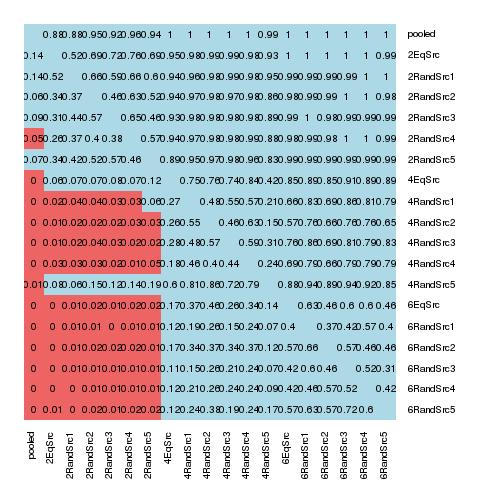
\includegraphics[width=\linewidth]{images/heatmapBC}
  \caption{Validity}
  \label{fig:valBC}
\end{subfigure}%
\begin{subfigure}{.5\textwidth}
  \centering
  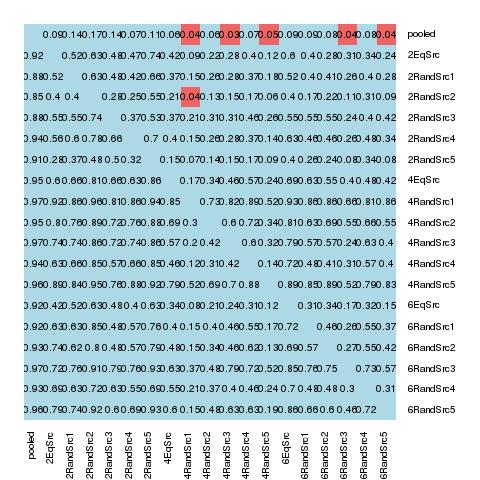
\includegraphics[width=\linewidth]{images/heatmapBC_eff}
  \caption{Efficiency}
  \label{fig:effBC}
\end{subfigure}%
\caption{Results of statistical tests with BC data. All significant p-values are marked in red.} \label{fig:testBC}
\end{figure}

\subsection{Empirical results on Spambase data}
This is a data set with 4601 observations on 57 variables and 1 target class with spam or non-spam class labels. The following are the class distributions:

\begin{center} 

\begin{tabular}{l|c}
Class Label & \# of instances \\
\toprule
spam &  2788\\
non-spam &  1813\\
\end{tabular}
\end{center}

The results for comparing the different methods on Spambase data, by applying the Wilcoxon signed-rank test on validity and efficiency, are shown in subfigures (\ref{fig:valSpam}) and (\ref{fig:effSpam}) respectively, in Figure \ref{fig:testSpam}.



\begin{figure}[!h]
\centering
\begin{subfigure}{.5\textwidth}
  \centering
  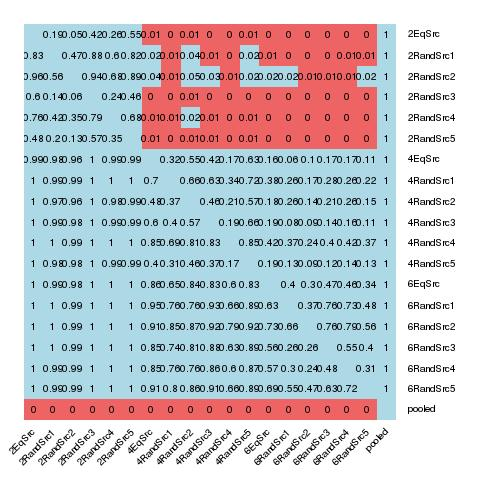
\includegraphics[width=\linewidth]{images/heatmapSpam}
  \caption{Validity}
  \label{fig:valSpam}
\end{subfigure}%
\begin{subfigure}{.5\textwidth}
  \centering
  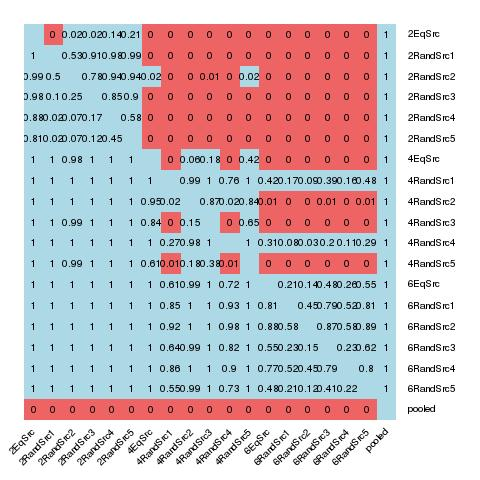
\includegraphics[width=\linewidth]{images/heatmapSpam_eff}
  \caption{Efficiency}
  \label{fig:effSpam}
\end{subfigure}%
\caption{Results of statistical tests with Spambase data. All significant p-values are marked in red.}
\label{fig:testSpam}
\end{figure}

\newpage

\subsection{Empirical results on Mushroom data}
This is a data set with 8124 observations on 21 variables and 1 target class with edible or non-edible class labels. The following are the class distributions:

\begin{center} 

\begin{tabular}{l|c}
Class Label & \# of instances \\
\toprule
spam &  3916\\
non-spam &  4208\\
\end{tabular}
\end{center}

The results for comparing the different methods on Mushroom data, by applying the Wilcoxon signed-rank test on validity and efficiency, are shown in subfigures (\ref{fig:valMush}) and (\ref{fig:effMush}) respectively, in Figure \ref{fig:testMush}.

\begin{figure}[!h]
\centering
\begin{subfigure}{.5\textwidth}
  \centering
  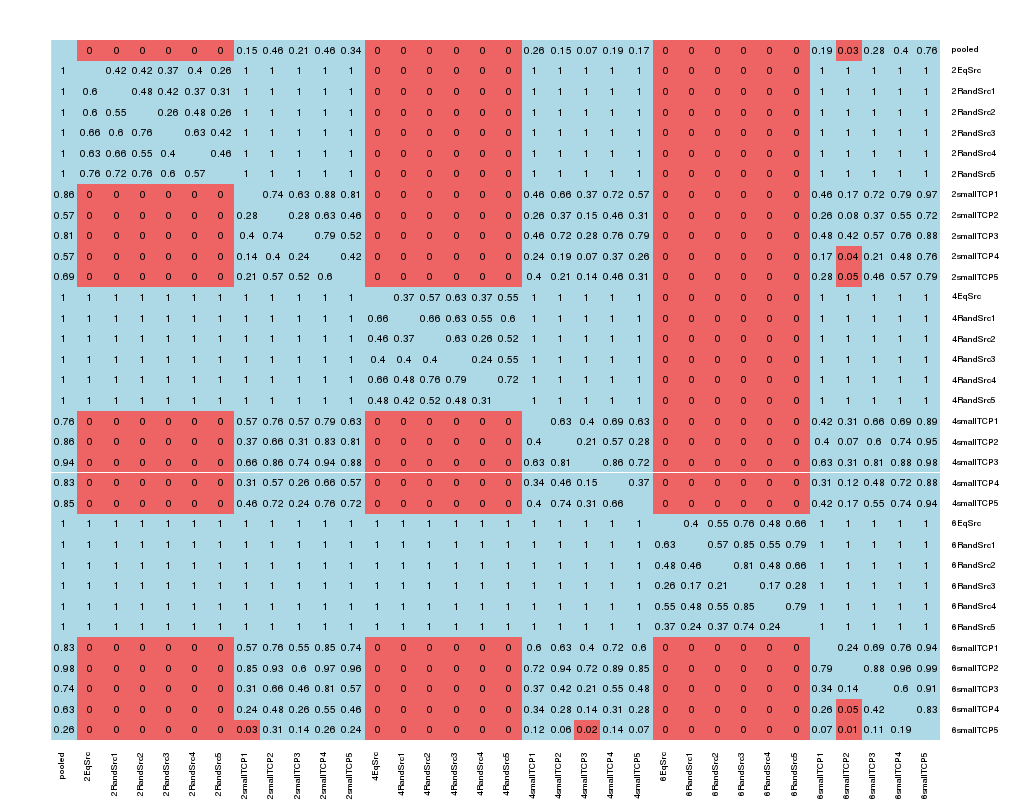
\includegraphics[width=\linewidth]{images/heatmapMush}
  \caption{Validity}
  \label{fig:valMush}
\end{subfigure}%
\begin{subfigure}{.5\textwidth}
  \centering
  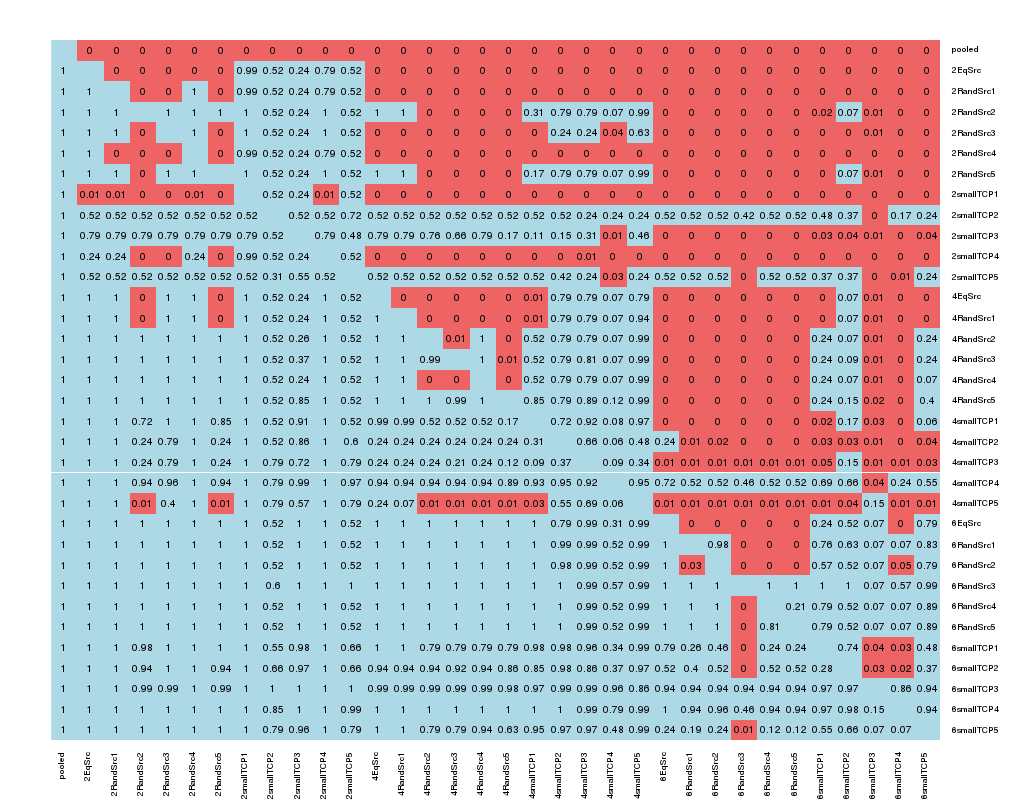
\includegraphics[width=\linewidth]{images/heatmapMush_eff}
  \caption{Efficiency}
  \label{fig:effMush}
\end{subfigure}%
\caption{Results of statistical tests with Mushroom data. All significant p-values are marked in red.} \label{fig:testMush}
\end{figure}

\subsection{Empirical results on FOTP data}
The First Order Theorem Proving (FOTP) is a real data set with 4587 observations (actual training and test sets used) on 51 variables and 1 target class with +1 where no heuristic finds a   proof within the time limit and -1 otherwise.  The following are the class distributions:

\begin{center}

\begin{tabular}{l|c}
Class Label & \# of instances \\
\toprule
proof within the time limit &  1909\\
proof within the time limit &  2678\\
\end{tabular}
\end{center}

The results for comparing the different methods on FOTP data, by applying the Wilcoxon signed-rank test on validity and efficiency, are shown in subfigures (\ref{fig:valFotp}) and (\ref{fig:effFotp}) respectively, in Figure \ref{fig:testFotp}.

\begin{figure}[!h]
\centering
\begin{subfigure}{.5\textwidth}
  \centering
  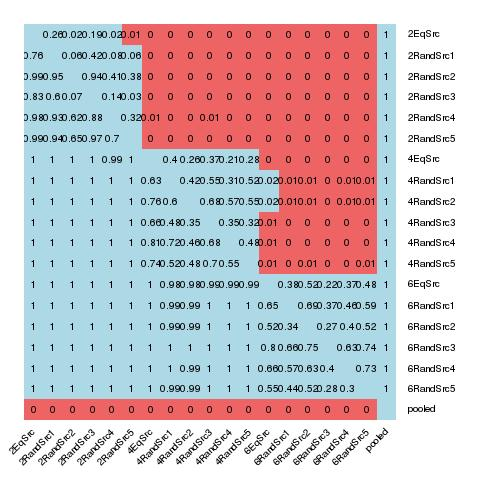
\includegraphics[width=\linewidth]{images/heatmapFotp}
  \caption{Validity}
  \label{fig:valFotp}
\end{subfigure}%
\begin{subfigure}{.5\textwidth}
  \centering
  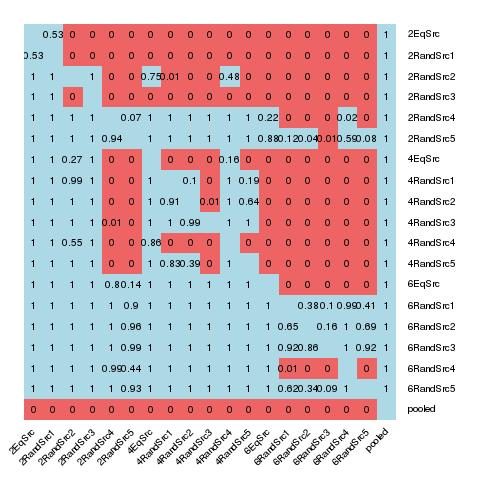
\includegraphics[width=\linewidth]{images/heatmapFotp_eff}
  \caption{Efficiency}
  \label{fig:effFotp}
\end{subfigure}%
\caption{Results of statistical tests with FOTP data. All significant p-values are marked in red.} \label{fig:testFotp}
\end{figure}

\subsection{Empirical results on Phishing Website data}
The Fishing Website is a real data set with 2455 observations  on 30 variables and 1 target class with 1 as legitimate and 2 as suspicious class labels.  The following are the class distributions:

\begin{center}

\begin{tabular}{l|c}
Class Label & \# of instances \\
\toprule
legitimate &  1362\\
suspicious &  1093\\
\end{tabular}
\end{center}

The results for comparing the different methods on Phishing Website data, by applying the Wilcoxon signed-rank test on validity and efficiency, are shown in subfigures (\ref{fig:valPhish}) and (\ref{fig:effPhish}) respectively, in Figure \ref{fig:testPhish}.

\begin{figure}[!h]
\centering
\begin{subfigure}{.5\textwidth}
  \centering
  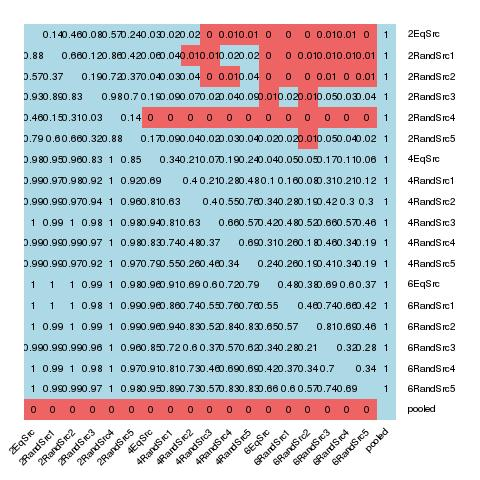
\includegraphics[width=\linewidth]{images/heatmapPhish}
  \caption{Validity}
  \label{fig:valPhish}
\end{subfigure}%
\begin{subfigure}{.5\textwidth}
  \centering
  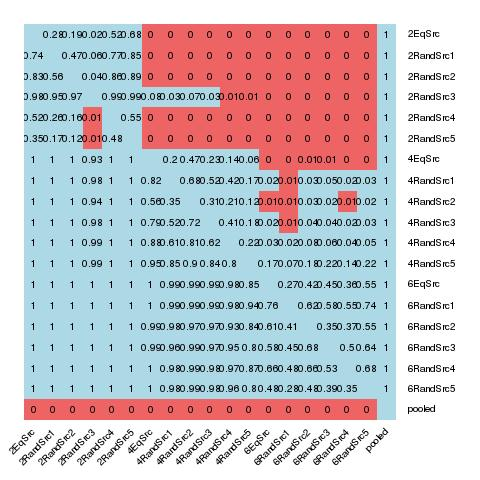
\includegraphics[width=\linewidth]{images/heatmapPhish_eff}
  \caption{Efficiency}
  \label{fig:effPhish}
\end{subfigure}%
\caption{Results of statistical tests with Phishing Website data. All significant p-values are marked in red.} \label{fig:testPhish}
\end{figure}

\newpage

\subsection{Empirical results on Combined data}

\begin{figure}[!h]
\centering
\begin{subfigure}{.5\textwidth}
  \centering
  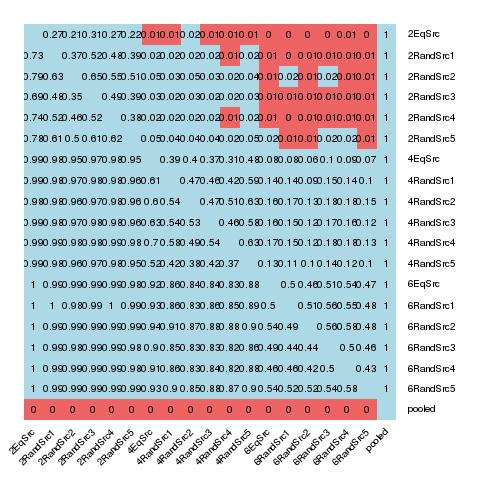
\includegraphics[width=\linewidth]{images/heatmapCombined}
  \caption{Validity}
  \label{fig:valCombined}
\end{subfigure}%
\begin{subfigure}{.5\textwidth}
  \centering
  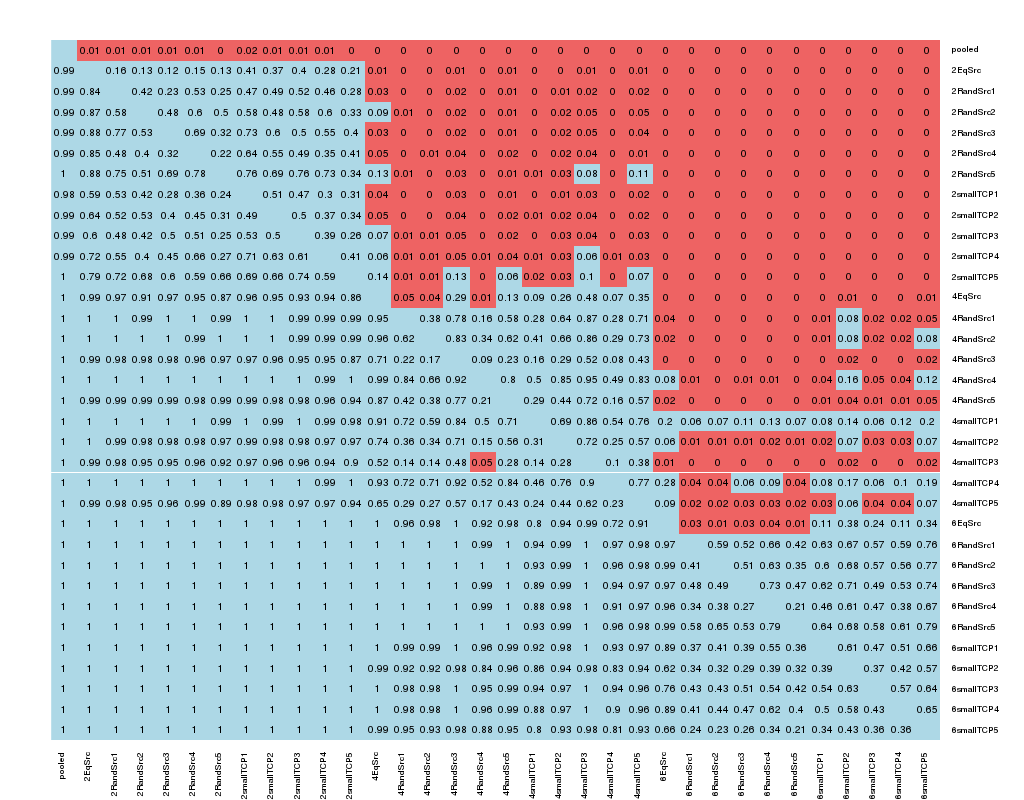
\includegraphics[width=\linewidth]{images/heatmapCombined_eff}
  \caption{Efficiency}
  \label{fig:effCombined}
\end{subfigure}%
\caption{Results of statistical tests with combining all the data. All significant p-values are marked in red.} \label{fig:testCombined}
\end{figure}

 









 

\end{document}
